\documentclass[12pt,letterpaper]{article}

\usepackage{amsmath, amsthm, amsfonts, amssymb}
\usepackage{microtype, parskip, graphicx}
%\usepackage[comma,numbers,sort&compress]{natbib}
\usepackage[style=numeric-comp,
      backend=biber,
      bibencoding=utf8,
      maxbibnames=10,
      uniquename=init,
      giveninits=true,
      sorting=none,
      natbib=true,
      url=false,
      doi=false,
      isbn=false]{biblatex}
\usepackage[margin=1in]{geometry}
\usepackage{lineno}
\usepackage{longtable}
\usepackage{caption, subcaption, multirow, morefloats, rotating}
\usepackage{wrapfig}
\usepackage{hyperref}
\usepackage{threeparttable}

\frenchspacing


\newcommand{\beginsupplement}{
 \setcounter{section}{0}
 \renewcommand{\thesection}{S\arabic{section}}
 \setcounter{table}{0}
 \renewcommand{\thetable}{S\arabic{table}}
 \setcounter{figure}{0}
 \renewcommand{\thefigure}{S\arabic{figure}}
 \setcounter{equation}{0}
 \renewcommand{\theequation}{S\arabic{equation}}
}

% https://3d.bk.tudelft.nl/hledoux/blog/fiddling-biblatex/
%-- formatting hell for biblatex
%-- remove "In:"
\renewbibmacro{in:}{}
%-- no "quotes" around titles of chapters/article titles
\DeclareFieldFormat[article, inbook, incollection, inproceedings, misc, thesis, unpublished]
{title}{#1}
%-- no punctuation after volume
\DeclareFieldFormat[article]{volume}{ {#1} } 
%-- puts number/issue between brackets
\DeclareFieldFormat[article, inbook, incollection, inproceedings, misc, thesis, unpublished]{number}{\mkbibparens{#1}} 
%-- and then for articles directly the pages w/o any "pages" or "pp." 
\DeclareFieldFormat[article]{pages}{#1}
%-- for some types replace "pages" by "p."
\DeclareFieldFormat[inproceedings, incollection, inbook]{pages}{p. #1}

% https://tex.stackexchange.com/questions/81569/biblatex-parentheses-around-the-volume-number-of-an-article
\renewbibmacro*{volume+number+eid}{%
 \printfield{volume}%
 \printfield{number}%
 \printfield{eid}}
\DeclareFieldFormat[article]{number}{\mkbibparens{#1}}


% bibliographic information
%\bibliographystyle{abbrvnat}
%\bibliography{citations}
\addbibresource{citations.bib}

\title{How predictable is extinction? Forecasting species survival at million-year timescales}
\author{
 Smits, Peter\\
 %Department of Integrative Biology, University of California Berkeley\\
 \texttt{psmits@berkeley.edu} 
 \and
 Finnegan, Seth\\
 %Department of Integrative Biology, University of California Berkeley\\
 \texttt{sethf@berkeley.edu}
}
\date{}

\begin{document}
\beginsupplement
\begin{refsection}

%\section{Supplemental Figures}

\setcounter{page}{1}
\section{Supplement to Materials and Methods}

\subsection{Data Specifications} \label{sec:data_desc}

\subsubsection{Binning fossil occurrences}

The estimated age of each occurrence is based on the core-specific age-model that observation is from and can be overly precise. To alleviate this overprecision, we coarsened our temporal information in an effort to limit the effects of between-core heterogeneity in age. The occurrence histories of each species was then summarized as a series of binary codes indicating the presence or last occurrence of that species. For every occurrence of a species, except the last, that species existence and survival is recorded as a 0. The last occurrence of that species is considered the bin in which the taxon has gone extinct -- and is recorded as 1. This protocol means that we are reading the fossil record ``as written,'' a practice that is potentially dangerous as it is an overconfident statement of preservation and may be shortening the actual durations of the studied species \citep{Alroy2010,Alroy2000b,Alroy2014,Foote1997,Foote1999a,Foote2001,Foote1996e,Lloyd2012b,Marshall1995,Wang2016}. However, this practice is common with marine microfossil data due to their exceptional preservation rate \citep{Ezard2013,Ezard2016,Ezard2011,Liow2010}. In fact, with marine microfossils collected from cores a bigger problem may be over extending the duration of a species due to mixing and smearing within the cores \citep{Mekik2018,Broecker1999,Mekik2014,Peng1984}.


\subsubsection{Covariate transformation and standardization}

Prior to analysis, geographic range was then log-plus-one transformed and standardized by mean-centering the data and then dividing by the standard deviation of the distribution of geographic ranges. This standardization means that a regression coefficient associated with each covariate describes the change in extinction probability per change in standard deviation of that covariate, that coefficients associated with similarly standardized covariates will be directly comparable in magnitude, and that the intercept term corresponds to the expected value of the outcome at when geographic range is its average value \citep{ARM}. Change in geographic range between observations was measured from the standardized geographic range values and was not standardized separately.

Temperature was also transformed and standardized the in the same manner as geographic range. The change in temperature between an observation and its previous observation was measured from the standardized temperature values and was not standardized separately.


\subsection{Model Specifications} \label{sec:model_desc}

In survival analysis, the hazard function describes the instantaneous rate of extinction of a species given its age and covariate information. The hazard function is defined as the conditional probability of a species going extinct by the end of the \(t\)-th interval given that it survived up until \(t\) and the relevant covariate information \(X\) for all \(k\) 1 My intervals \citep{Tutz2016}. For the discrete time intervals \(T = 1, \cdots, k\), extinction is defined as \(T = t\). The discrete time hazard function is defined as
\begin{equation}
 \lambda(t | X) = P(T = t | T \geq t, X), \quad t = 1, \cdots, k.
 \label{eq:hazard}
\end{equation}

The hazard function (Eq. \ref{eq:hazard}) is easily reparameterized as a logistic regression by defining that \(\lambda(t | X) = h(\Theta)\) where \(h(.)\) is a logit inverse-link function and \(\Theta\) is the probability of a taxon going extinction during interval \(t\) \citep{Tutz2016}. \(h(\Theta)\) is then modeled as with any regression. In this case, we opted for a hierarchical/mixed-effects model with multiple non-nested varying intercepts and slopes \citep{ARM}.

Our covariates matrix \(X\) is a \(N \times D\) matrix where \(N\) is the total number of observations and \(D\) is the total number of covariates. The first column of \(X\) is entirely 1's as it corresponds to the intercept term in the regression model. The next two columns of \(X\) are two aspects of geographic range as continuous covariates: geographic range \(r\) during interval \(t\), and the difference \(d\) between the geographic range at \(t - 1\) and \(t\). Change in geographic range was calculated from the transformed and standardized geographic range values; this means that change in geographic range is in units of changes in standard deviations. The final two columns are two aspects of global temperature: mean temperature during interval \(t\), and the lag of mean temperature (i.e. mean temperature during interval \(t - 1\).) As with change to geographic range, the lag of temperature is based on the transformed and standardized temperature estimates. 

The matrix of time and phylum varying regression coefficients describing the effects of the covariates on a species' risk of extinction is called \(B\) -- a \(w\) by \(p\) matrix, were \(w\) is the number of time temporal intervals and \(p\) is the number of phyla. The elements of this matrix, the regression coefficients, are themselves modeled as being multivariate normally distributed with vector of means \(\alpha\) describing the average intercept and regression coefficient estimates of each phylum \(p\). These phylum averages are themselves modeled as multivariate normally distributed with mean vector \(\mu\) describing the overall average regression coefficients, including the intercept. \(\mu\) has length \(D\) and is ordered intercept, range coefficient, change in range coefficient, temperature coefficient, temperature lag coefficient.

The effect of species age on the log-odds of species extinction is modeled as a non-nested random intercept \(A\) \citep{Tutz2016}. This term describes how the log-odds of extinction varies along a species duration, and how this effect can differ between the phyla. \(A\) is a \(l\) by \(p\) matrix, where \(l\) is the age at observation of a species and \(p\) is its phylum. \(A\) is modeled as following a multivariate normal distribution with phylum means being the vector \(\delta\) and covariance matrix \(\Sigma_{A}\). The covariation between the elements of vector \(\delta\) are modeled as a multivariate normal distribution with a mean vector of all 0s and covariance matrix \(\Sigma_{\delta}\).

To complete the generative model, we need to assign final priors to the ``top-level'' parameters. In general, we favored weakly informative priors which help regularize our estimates. In the case of a regression coefficient, this means a Normal distribution with mean 0 and a standard deviation of 3. For our scale parameters (e.g. standard deviations), we used half-Cauchy distributed priors with heavy tails but the majority of probability density near 0.

Our top-level intercept was given a more diffuse prior than our regression coefficients, which reflects our greater degree of uncertainty about its value. Our top-level regression coefficient for the effect of geographic range was given an informative prior reflecting the overwhelming amount of evidence that species with a larger than average geographic range have a lower risk of extinction than species with an average or less than average geographic range. In the context of this analysis, this means that we are again using a weakly informative prior but instead of centering the density around -1 (i.e. larger than average geographic range decreases extinction risk).

Instead of assigning a prior distribution for each of the covariance matrices in the model, we instead decomposed the covariance matrices (e.g. \(\Sigma_{B}\)) which allows us to assign independent priors for the scale and correlation aspects of covariance. The scale parameters were assigned half-Cauchy priors as described above in the context of all other scale parameters. The correlation matrices were assigned LKJ priors each with shape parameter set to 1. This choice of shape parameter produces a uniform distribution over possible correlation matrices. These priors are also slightly more interpretable than other common prior distributions for covariance matrices such as the inverse-Wishart distribution. This approach to assigning priors to a covariance matrix is recommended by the Stan Manual \citep{StanManual}.

In total, our model can be expressed as: 
\begin{equation}
 \begin{aligned}
  t_{i} &\sim \text{Bernoulli}(\Theta) \\
  \Theta_{i} &= \text{logit}^{-1} (X_{i} B_{w[i], p[i]} + A_{l[i], p[i]}) \\
  B_{w, p} &\sim MVN(\alpha_{p}, \Sigma_{B}) \\
  \alpha_{p} &\sim MVN(\mu, \Sigma_{\alpha}) \\
  % double check this\dots is A MVN dist?
  A_{l, p} &\sim MVN(\delta_{p}, \Sigma_{A}) \\
  \delta_{p} &\sim \mathrm{N}(0, \sigma_{\delta}) \\
  \mu_{d} &\sim 
  \begin{cases}
   N(-2, 5) & \text{if } d = \text{intercept} \\
   N(-1, 1) & \text{if } d = \text{geo. range} \\
   N(0, 1) & \text{else } \\
  \end{cases} \\
  \delta &\sim N(0, 1) \\
  \Sigma_{B} &= diag(\tau_{B}) \Omega_{B} diag(\tau_{B}) \\
  \Sigma_{\alpha} &= diag(\tau_{\alpha}) \Omega_{\alpha} diag(\tau_{\alpha}) \\
  \Sigma_{A} &= diag(\tau_{A}) \Omega_{A} diag(\tau_{A}) \\
  \tau_{B} &\sim C^{+}(1) \\
  \tau_{\alpha} &\sim C^{+}(1) \\
  \tau_{A} &\sim C^{+}(1) \\
  \Omega_{B} &\sim LKJ(1) \\
  \Omega_{\alpha} &\sim LKJ(1) \\
  \Omega_{A} &\sim LKJ(1) \\
 \end{aligned}
 \label{eq:model}
\end{equation}
with \(i\) indexing the observation and bracket subscripts referencing the class of the \(i\)th observation where \(w[i]\) is the time of the \(i\)-th observation, \(p[i]\) is the phylum of the \(i\)-th observation, and \(d[i]\) is the age of the \(i\)-th observation. 


\subsection{Model Parameter Estimation} \label{sec:model_est}

We implemented our model (Eq. \ref{eq:model} using the \begin{texttt}rstanarm\end{texttt} package for the R programming language \citep{StanManual}. This package provides an interface to the Stan probabilistic programming language for writing hierarchical/mixed-effects models in native R. Posterior estimates were obtained through Hamiltonian Monte Carlo, using 2000 steps divided equally between warm-up and sampling. In order to prevent divergent transitions adapt delta was increased to 0.999999; all other HMC/NUTS sampling parameters were kept at the defaults for rstanarm 2.18.2 \citep{rstanarm}.

To implement our VP model in \begin{texttt}rstanarm\end{texttt}, where ``data'' is a data.frame object of all necessary data (response, covariates), is coded as:
\begin{verbatim}
form <- event ~ 
        range + range_diff1 + range_diff2 + range_diff3 + 
        temp + temp_lag + 
        (1 + range + range_diff + temp + temp_lag | mybin/phylum) + 
        (1 | age/phylum), 
stan_glmer(formula = form,
      data = data, 
      family = 'binomial',
      prior = normal(c(-1, 0, 0, 0, 0, 0), rep(1, 6), autoscale = FALSE), 
      prior_intercept = normal(-2, 5, autoscale = FALSE), 
      prior_aux = cauchy(0, 1, autoscale = FALSE), 
      chains = 4,
      thin = 4,
      adapt_delta = 0.999999)
\end{verbatim}

Similarly, our VP model can be implemented using the \begin{texttt}brms\end{texttt} Stan interface \citep{brms2017,brms2018} as:
\begin{verbatim}
priors <- c(set_prior('normal(-2, 5)', class= 'Intercept'),
      set_prior('normal(0, 1)', class = 'b'),
      set_prior('normal(-1, 1)', class = 'b', coef = 'range'),
      set_prior('cauchy(0, 1)', class = 'sd'),
      set_prior('lkj(1)', class = 'cor'))
form <- bf(event ~ 
           range + range_diff1 + range_diff2 + range_diff3 + 
           temp + temp_lag +
           (1 + range + range_diff + temp + temp_lag | mybin/phylum) +
           (1 | age/phylum))
brmfit <- brm(formula = form,
       data = data, 
       family = bernoulli(), 
       prior = priors,
       chains = 4, 
       thin = 4,
       control = list(adapt_delta = 0.999999)
\end{verbatim}

Posterior convergence was determined using the general and HMC-specific diagnostic criteria: scale reduction factor (\(\hat{R}\); target \(<1.1\)), effective sample size (eff; target value eff/steps \(<0.0001\)), number of samples that saturated the maximum trajectory length for avoiding infinite loops (treedepth; target value 0), sample divergence, and the energy Bayesian Fraction of Mission Information (E-BFMI; target value \(>0.2\)). For further explanation of these diagnostic criteria, see the Stan Manual \citep{StanManual}.

\section{Supplement to Results} \label{sec:supp_res}

Here we present the parameter estimates for our from our VP model (Table 1). We choose to present the estimates from this model because it is our most inclusive model and its parameter estimates are indicative of parameter estimates from other models with a subset of those covariates included in this model.

First, we present the group-level estimates of our regression coefficients and intercept (Fig. \ref{fig:param_est}). Group-level effects are the average effects of that covariate over time and across taxonomic groups. These estimates make up the vector $\mu$ described above. In addition to the average effect of our covariates, we also included the estimate of the group-level intercept, which is the average log-odds of extinction for an average observation over time and across taxonomic groups.

\begin{figure}[ht]
  \centering
  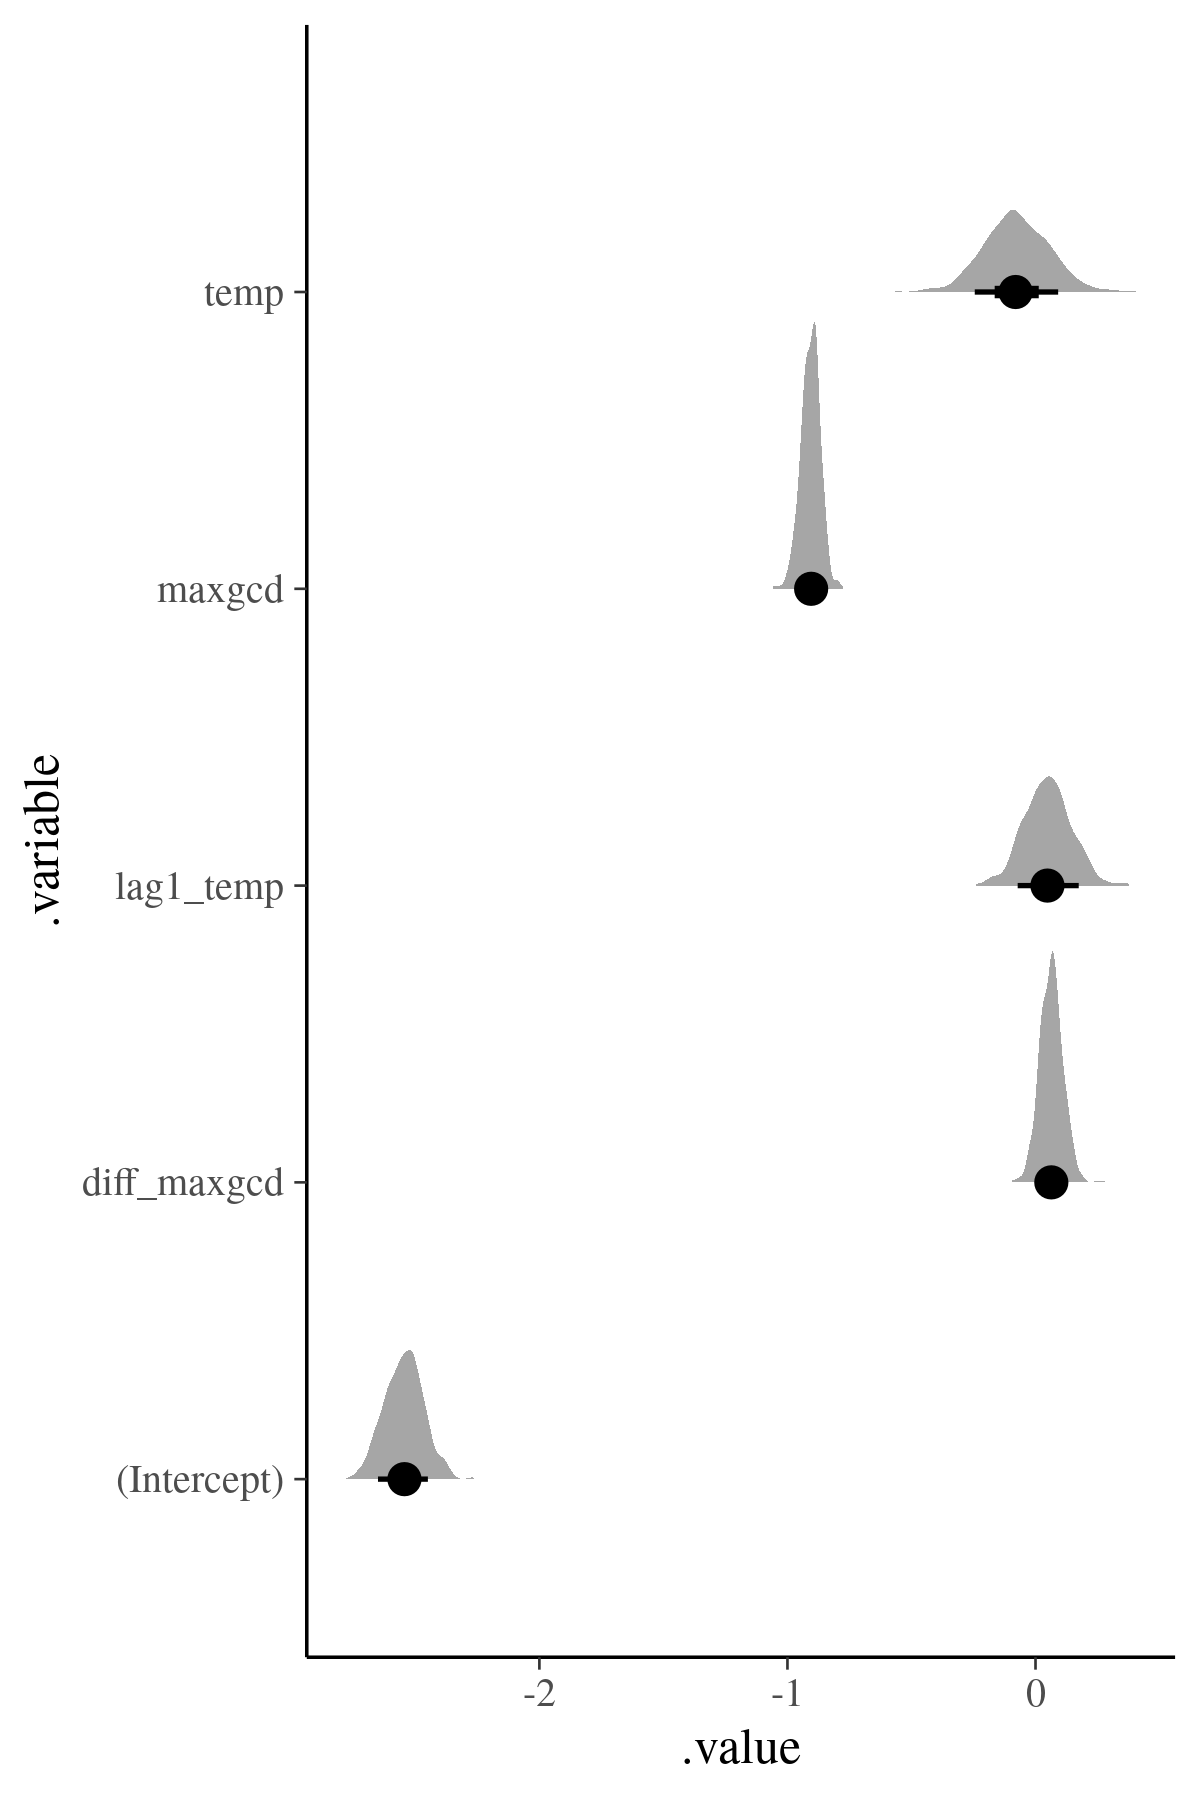
\includegraphics[width=\textwidth,height=\textheight,keepaspectratio=true]{../results/figure/effect_est}
  \caption{Group-level parameter posterior estimates from our VP model (Table 1). The posterior distribution of our parameter estimates are presented as densities. Below each of these densities is marked the median estimate along with 50\% and 80\% credible intervals. Estimates are on the log-odds scale.}
  \label{fig:param_est}
\end{figure}

Second, we present the population-level estimates for our regression coefficients along with the population-level intercept estimates (Fig. \ref{fig:param_est_time_group}. Our VP model allows for these our regression coefficients to vary over time and between taxonomic groups. Population-level estimates are those for a specific time interval and taxonomic group. In this case, the intercept estimate describes the log-odds of extinction for an average observation at that point in time and taxonomic group.

\begin{figure}[ht]
  \centering
  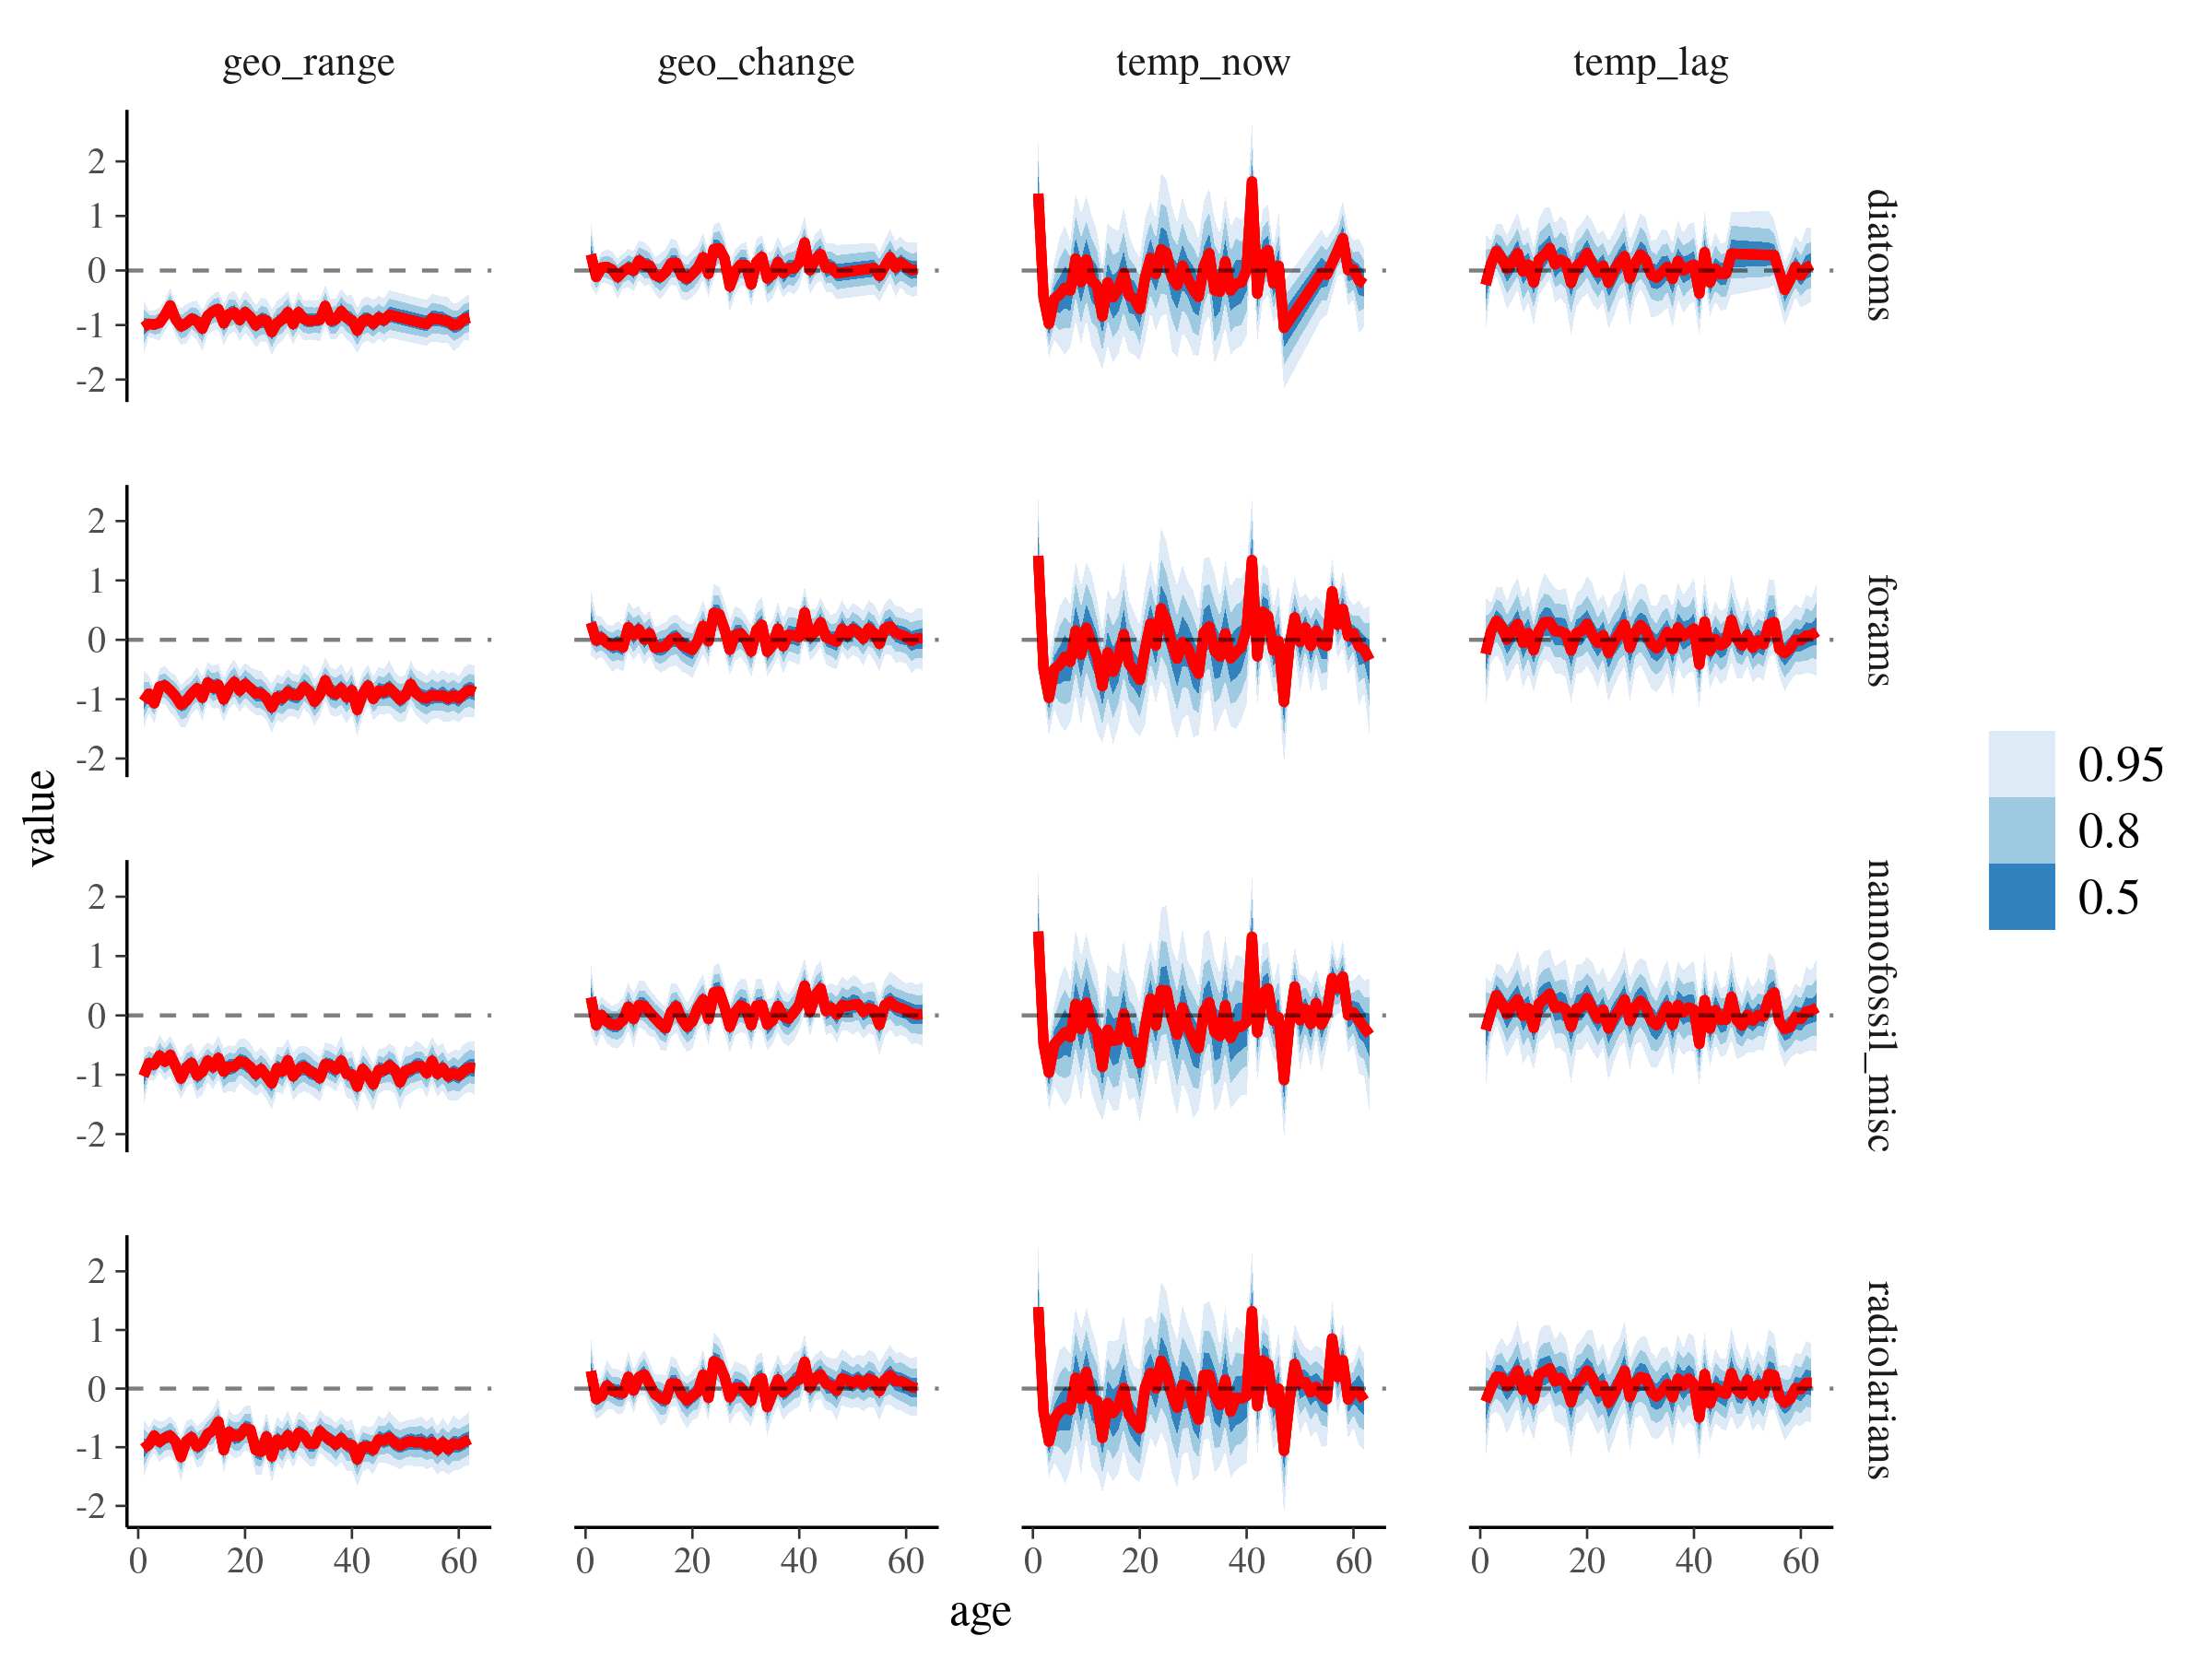
\includegraphics[width=\textwidth,height=\textheight,keepaspectratio=true]{../results/figure/eff_time_group}
  \caption{Population-level parameter posterior estimates from our VP model (Table 1). Posterior estimates are presented as a time series. The black line represents the median estimate of that parameter. In addition, the 50\%, 80\%, and 95\% credible intervals are indicated. Estimates are on the log-odds scale.}
  \label{fig:param_est_time_group}
\end{figure}



\printbibliography[title={Supplementary References}]
\end{refsection}

\end{document}


